%literature review
\section{Related prior work}

Relevant prior work fall into four rough categories. There is a large body of work on the subject of general automatic colour transfer and colour grading by example, transfering the ``style" or specific colours in an example image to another image. There have been several prior attempts at transfering color specifically for images wherein skin colour is prominent, and these we will discuss in detail. There are also several examples of practical application of skin transfer algorithms, where different application demonstrate practical uses of usually relatively simple skin transfer algorithm that is part of a larger project; we will discuss several of these projects. Finally, there is the field of skintone enhancement software, where algorithms are usually intended to adjust the user skin colour towards a more pleasing tone and not to a specific target colour. We include the latter because unlike the other categories of prior work there are several studies of adjusting skintone on a mobile device, which is part of the requirements for this project.

\section{Colour transfer by example image for general images}
Colour transfer refers to modifying the colours of an image to give it the desired appearance and style demonstrated by an example image, which we will refer to as the target image. Figure \ref{fig:color_transfer} illustrates an example of this effect.

There have been a wide range of work done in this area beginning with the seminal work of Reinhard et al. in 2001 \cite{reinhard_2001_transfer}. 

While these techniques are interesting possibilities to try when transfering human skin colour, because the these prior studies are all concerned with different problems that can arise with general images but not specifically for human skin colour, studies that specifically relate to human skin colour demonstrate that the general colour transfer techniques can be improved upon.

\section{Transfer of human skin colour}
Several studies have been done specifically on the transfer of human skin colour.

Seo et al. \cite{seo_2005_transfer} has a purpose closest to the purpose of this project, to transfer human skin colours. The authors show results that improve in realistic appearance compared to the Reinhard's algorithm.

% Models the skin as ellipsoid distribution around vector, with another vector for specular reflection
% Algorithm used - RGB space transform, division into bins and moving standard dev and mean while leaving details intact
% Results don't show range but we can possibly replicate and check?

It is not clear how fast the algorithm can run particularly on a mobile device, nor the range of colours that the algorithm can transform a single skin colour, and it is in these areas that our project will attempt to improve upon.

Yang et al. performed the most recent study of colour transfer for human portraits \cite{yang_2015_semantic}. However, this study focuses on the effect on the whole image, and places emphasis on transfering colour for different features of the human face. The actual algorithm used to transfer skin colour remains Reinhard's algorithm. This method also ranks the preferred target image for similarity to the original image before performing the colour transfer, which differs from our project where a key issue is that we have no control over the target image that the user will provide us. 

Yin et al. performed a study on the transfer of skin colour between races in order to aid a psychological study \cite{yin_2004_transfer}. 

% Study has flaws: quality of transfer - bright spots, realism for transfer from a lighter or midtoned skin colour to darker skin colour, and time taken to perform the transfer

We include this study because it is one of the few that explicitly tries to transfer colour between a large difference of skin colour.

\section{Skin colour transfer as part of other applications}
Several applications performing different functions make use of skin colour transfer.

Shilkrot et al. published a study on transfering identity of the user on to a model image wearing garments the user may desire to purchase to create the virtual experience of the user trying on the garment \cite{shilkrot_2013_garment}. The purpose of this article is fundamentally related to the purpose of the application that is this project's goal to support, and so this article is of great interest to us. 

In fact, as part of the identity transfer, this article performs skin colour transfer on the model image to take on the skin colour of the user. Shilkrot uses a Gaussian Mixed Model for transfer skin colours and seems to use it for a relatively wide range of color differences.
%explain this model
%Is there user interaction?
%timing wise, how fast?
%include figures of results

The difference between Shilkrot's study and ours is that skin is only a small part of their final image, and the skin transfer process is only a small part of their study, which also places emphasis on the transfer of the user's head and the reshaping of the model's body proportions. In our case, the hand will be the only object of interest in our inputs and outputs. While we need not devote our efforts to any aspect but the skin colour change, any flaws in the color transfer causing unrealistic results will be much more noticeable. 
% Are there other identity transfer articles?

Another interesting case of skin colour matching is the work Bitouk et al to create a face swapping software that seamlessly changes faces in photos to stock photo faces \cite{bitouk_2008_faceswap}. Since the skin colour of stock photo face does not exactly match the rest of the skin colour in the original photo, the authors adjust the lighting and skin colour until they do match. In their case however, the author specifically state large skin colour changes cannot be made, and to support a wide range of skin colours, the authors rely on having a large library of stock photos of every lighting position and skin colour. On the other hand, in our case, we are motivated by that fact that it is difficult to prepare videos for the full range of user skin colours.
%but it's fast though, should mention that

Another application we've found is the work Baba et al. to develop a software that edits portraits in yearbook photos to all have a uniform skin colour given an example skin colour image \cite{baba_2015_yearbook}. The algorithm that the authors use to acheive this uses Pitié's colour grading algorithm and guided image filtering. However, the goal of the project in terms of skin colour appears to be to have skin colours close to the target image but not necessarily exactly the same; the authors are focusing on the overall appearance of the set of portraits rather than the accuracy of the skin colour transfer for each individual image. On the other hand, the goal of our project is to ensure that the transformed skin colour of the model is as accurate as possible to the user's skin colour.
%explain guided image filtering

\section{Skin colour enhancement mobile applications}
For the most part the studies we have found are not meant to be run on a mobile platform and there are few specifically devoted to human skin colour. There are however many skin colour enhancement applications that modify human skin colour and several studies that perform this on mobile devices. 
%This makes sense as mobile devices all have cameras and these days skin tone enhancement is part of the functionality of the camera
%exceptions though - which algorithms are fast? garment,
%are you sure there are no other skin color change stuff on mobile platform? look more into this
%Mention the 2 studies at least
The difference between those studies and ours is that we have a target colour that could be very different from the colour that skin enhancement is aiming for, and our requirements for accuracy to the target colour is more stringent.

\section{Summary of differences between prior studies and this project}
Accuracy of colour transfer, use of a target image, nuances of colour transfer, speed of the colour transfer on a mobile device, range of colour transfer
%explain theoretical concepts in context of thesis work; be clear and concise
%summarize relevant research to give understanding of current field
%analyze research in field to give deeper understanding of research question 
%indicate a path going forward

%photoshop
\subsection{Changing and matching skin colour in Photoshop}

Skin colour correction is a frequent problem encountered in photo retouching and there are a wide range of online video tutorials available documenting the methods artists use to manually adjust human skin tone in individual images using Adobe Photoshop, a widely used commercial image manipulation software. The purposes of these videos include giving the subject of an image the appearance of a tan, matching the skin tone of the subject to a desired skin tone on another individual, or matching the skin tone of a subject's face to the rest of the subject's body, which is often a slightly different colour \cite{photoshop:tan, photoshop:match_other, photoshop:match_body}. Bearing in mind that techniques described by such tutorials expect artistic input from a human editor to acheive the results and are therefore not entirely aligned with the purposes of this project, it is useful to study these methods because the results achieved are usually extremely realistic and aesthetically pleasing and should be a standard that the algorithm developed in this project strives towards. We therefore surveyed a number of these videos and summarize below the techniques of some of the most relevant videos.

\subsubsection*{Summary of Photoshop techniques}

Shaver demonstrated how to change a person's skin colour from dark to light \cite{photoshop:obama}, which is an impressively wide range to change. Shaver used levels and curves, which are tools that manipulate the $rgb$ colour histogram of the image, to increase brightness to an extent, then performed further brightening by using a grey scale conversion to brighten the skin area of a black and white image and then using the luminosity blend mode to place the colour back into the image. We show the results acheived in Table \ref{tab:obama_demo}.

\begin{longtable}{|c|c|}
    \caption{Screen captures from Photoshop tutorial for changing skin colour from dark to light. \label{tab:obama_demo}}\\
    \hline
    Original & Result \\
    \hline
  \begin{minipage}{.29\textwidth}
    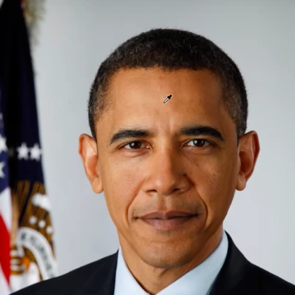
\includegraphics[width=\textwidth,height=\textheight,keepaspectratio]{images/obama_orig}
  \end{minipage} & 
  \begin{minipage}{.29\textwidth}
    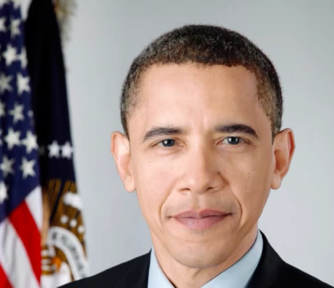
\includegraphics[width=\textwidth,height=\textheight,keepaspectratio]{images/obama_res}
  \end{minipage} \\
    \hline
\end{longtable}

Phlearn demonstrated an effect in the reverse direction by demonstrating a technique for giving the model the image appearance of a dark tan \cite{photoshop:tan}. The highlights and shadows of the image are adjusted separately by using the ``blend if" function of Photoshop, which blends in an effect only if the original pixel is above a certain threshold of brightness.

Phlearn also demonstrated a method for matching the skin colour of body and face in an image where the two appear mismatched \cite{photoshop:match_body}. The author sampled a range of colours from the body and adjusted the face with the levels tool for each colour channel. We show the results acheived in Table \ref{tab:match_body_demo}.

\begin{longtable}{|c|c|c|}
    \caption{Screen captures from Photoshop tutorial for matching the skintones of face and body. \label{tab:match_body_demo}}\\
    \hline
    Original & Target & Result \\
    \hline
  \begin{minipage}{.29\textwidth}
    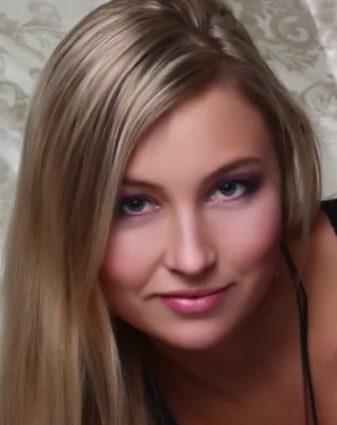
\includegraphics[width=\textwidth,height=\textheight,keepaspectratio]{images/match_body_orig}
  \end{minipage} & 
  \begin{minipage}{.29\textwidth}
    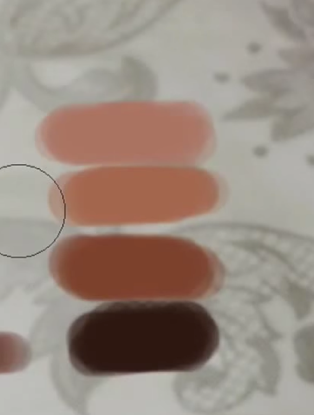
\includegraphics[width=\textwidth,height=\textheight,keepaspectratio]{images/match_body_targ}
  \end{minipage} & 
  \begin{minipage}{.29\textwidth}
    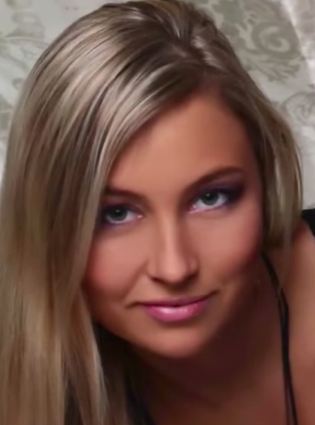
\includegraphics[width=\textwidth,height=\textheight,keepaspectratio]{images/match_body_res}
  \end{minipage} \\
    \hline
\end{longtable}

PiXimperfect demonstrated a method for matching skin colour in one portrait to another \cite{photoshop:match_other}. PiXimperfect first calculates the two average colours of the faces and uses the Photoshop curves tool to match the average colours of the original image to the target image. There must then be further adjustments by eye to change colour, brightness and contrast. Examples of the results from PiXimperfect is show in Table \ref{tab:match_other_demo}

\begin{longtable}{|N||c|c|c|}
    \caption{Screen captures from Photoshop tutorial for matching the skintones of portraits of different people. \label{tab:match_other_demo}}\\
    \hline
    \multicolumn{1}{|c||}{No.} & Original & Target & Result \\
    \hline  \label{row:photoshop_match_other_1} &
  \begin{minipage}{.29\textwidth}
    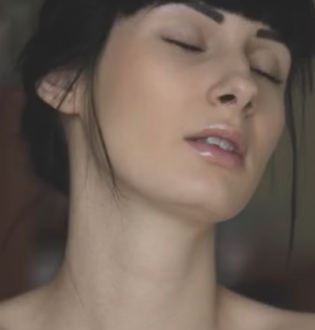
\includegraphics[width=\textwidth,height=\textheight,keepaspectratio]{images/match_other_1_orig}
  \end{minipage} & 
  \begin{minipage}{.29\textwidth}
    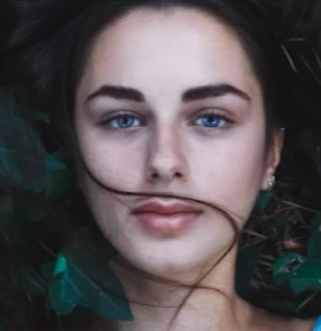
\includegraphics[width=\textwidth,height=\textheight,keepaspectratio]{images/match_other_1_targ}
  \end{minipage} & 
  \begin{minipage}{.29\textwidth}
    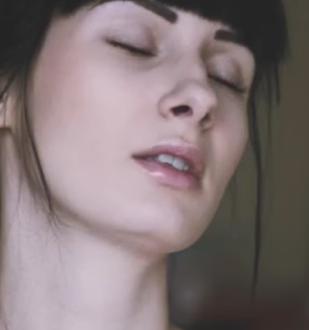
\includegraphics[width=\textwidth,height=\textheight,keepaspectratio]{images/match_other_1_res}
  \end{minipage} \\
    \hline  \label{row:photoshop_match_other_2} &
  \begin{minipage}{.29\textwidth}
    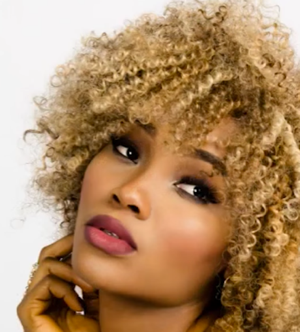
\includegraphics[width=\textwidth,height=\textheight,keepaspectratio]{images/match_other_2_orig}
  \end{minipage} & 
  \begin{minipage}{.29\textwidth}
    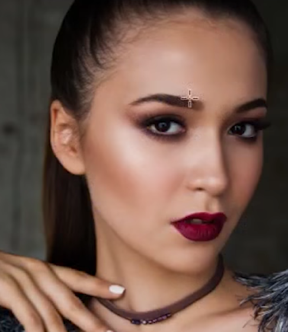
\includegraphics[width=\textwidth,height=\textheight,keepaspectratio]{images/match_other_2_targ}
  \end{minipage} & 
  \begin{minipage}{.29\textwidth}
    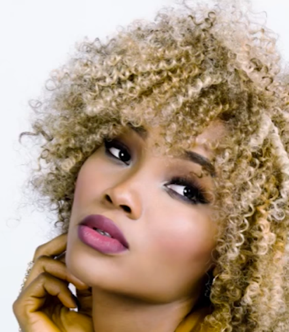
\includegraphics[width=\textwidth,height=\textheight,keepaspectratio]{images/match_other_2_res}
  \end{minipage} \\
    \hline
\end{longtable}

In summary, for most of the techniques surveyed, levels and curves are frequently used for small brightness adjustments \cite{photoshop:obama, photoshop:match_body, photoshop:match_other}, and often to reduce the vividness of the colour adjustments the saturation must be slightly decreased \cite{photoshop:obama, photoshop:match_body}. After all other effects are applied, the opacity of the overall effect is often reduced from 100\% for a more natural appearance \cite{photoshop:obama, photoshop:match_body}.

\subsubsection*{Limitations of Photoshop techniques}
Unlike the purpose of our project, the Photoshop techniques surveyed are not meant for automation. Instead, they are meant to be tailored to each specific image that a human is adjusting, and there are many junctures where the specific numerical amount of an adjustment often have to be judged by eye. While Photoshop has a method for automating processes using actions, the processes are meant for increasing ease of use by artists who can make additional adjustments and are familiar with the tool, rather than for use in commercial applications where the process is entirely automated \cite{photoshop:actions}.

Another limitation is that Photoshop operates at a higher level of abstraction than image processing software making use of libraries such as OpenCV. Image processing code has much more control over processes that can be applied to images, and the regions on the image that processes are applied to. 

Finally, some Photoshop effects may be proprietary and are of course limited to the platforms that Photoshop supports, while a program developed with a platform such as OpenCV can be made open source and adapted to uses on a variety of different platforms.
